\subsection{Esecuzione dell'esperienza}

La prima operazione fatta è stata quella di verificare il corretto allineamento dell'interferometro. Abbiamo infatti notato che se i due specchi non sono perpendicolari tra loro, sullo schermo si vedono figure di interferenza complicate e difficili da trattare invece che una semplice figura di interferenza lineare in cui si alternano massimi e minimi. Per allineare lo strumento è sufficiente ruotare delicatamente i due specchi finche non compare sullo schermo una figura d'interferenza semplice.

%Facciamo notare che nonostante l'attenzione prestata, lo specchio e lo schermo non sono risultati essere perfettamente paralleli tra di loro. Questo comporta che i due raggi luminosi incidenti sullo schermo non sono allineati tra di loro. Infatti sullo schermo si visualizzano in alternanza delle frange di interferenza costruttiva e distruttiva, ovvero picchi luminosi e non che si alternano con regolarità.
% WTF????

La misura dell'indice di rifrazione di un dato materiale con l'interferometro di Michelson si esegue adottando la seguente strategia.
Si parte da una configurazione base, per esempio l'interferometro con un ramo su cui e già stata montata la camera da vuoto
(si veda la Figura \ref{fig:mik}). A questo punto sullo schermo è proiettata una figura di interferenza. Dopodiché si
varia gradualmente un qualche parametro del materiale sotto esame, per esempio: la pressione (nel caso dell'aria), la lunghezza,
l'inclinazione oppure la concentrazione (per una soluzione). Questo serve per variare il cammino ottico del raggio che attraversa il materiale.
In questo modo la figura di interferenza varia e le frange si muovono.

%La seguente relazione lega il numero $N$ di frange passate sullo schermo, alla differenza di cammino ottico $d$.

%\begin{equation}
%    N \,=\, \frac{d}{\lambda} = \frac{\Delta n \cdot 2 \ell}{\lambda}
%\end{equation}
%
%Nella formula $\lambda$ indica la lunghezza d'onda della luce, $\Delta n$ la differenza di indice di rifrazione tra la configurazione base e quella attuale, mentre $2\ell$ e la lunghezza della camera (il 2 serve perché la luce attraversa la camera due volte).

%Una volta giunti al valore di pressione, lunghezza concentrazione voluto,


\begin{SCfigure}[0.70][t]
    \centering
    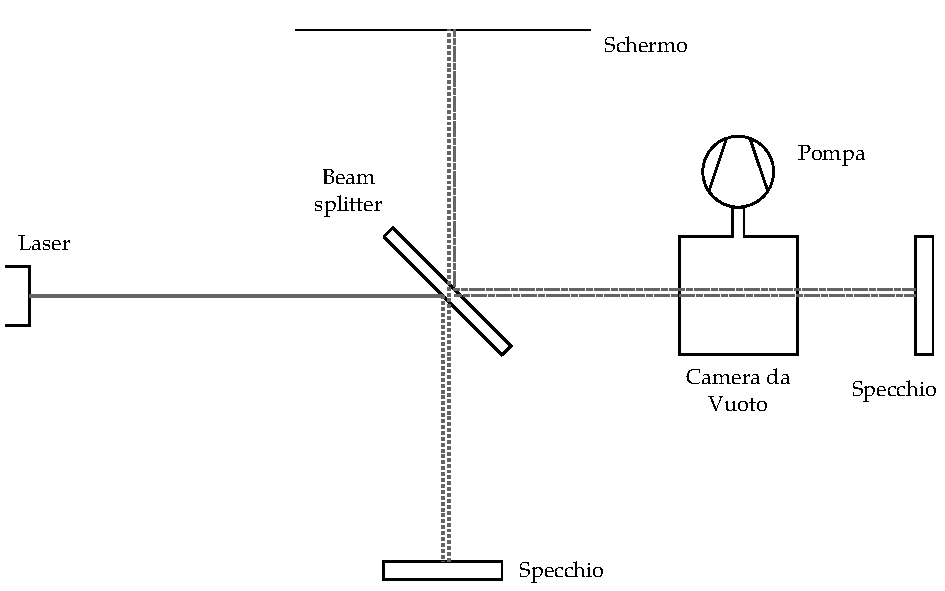
\includegraphics[width=120mm]{drawing.pdf}
    \caption{Schema semplificato del sistema utilizzato per misurare l'indice di rifrazione dell'aria.}
    \label{fig:mik}
\end{SCfigure}

\subsubsection{Indice di rifrazione dell'aria}

Detto questo la procedura eseguita per ricavare l'indice di rifrazione dell'aria è la seguente:

\begin{itemize}
	\item{Abbiamo installato sul sistema, tra il beam splitter e lo specchio mobile, una piccola camera da vuoto con due pareti in vetro atte a far passare la luce. La camera è stata collegata, mediante la valvola a spillo alla pompa a membrana;}
    \item{Partendo con la camera da vuoto a pressione atmosferica abbiamo man mano creato il vuoto all'interno della camera regolando l'apertura della valvola a spillo. Aprendo la valvola a spillo (ovviamente con la pompa accesa), l'aria esce dalla camera da vuoto e viene pompata fuori;}
    \item{Ad intervalli regolari di pressione, ovvero ogni \SI{10}{\kilo\pascal}, abbiamo annotato il numero di frange di interferenza passate sullo schermo;}
\end{itemize}

\subsubsection{Indice di rifrazione del vetro}

Per misurare l'indice di rifrazione del vetro abbiamo adottato una strategia simile. Dobbiamo partire da una data figura di interferenza e variare il cammino ottico di uno dei due raggi. Poi dobbiamo contare il numero di massimi di intensità (ovvero delle frange).

Infatti ponendo un vetro tra il beam splitter e lo specchio fisso si ottiene un effetto analogo a guello del caso precedete. Ovvero il raggio luminoso rifratto è costretto ad attraversare il vetro sia in andata che al ritorno e quindi subirà un variazione del suo cammino ottico.
Quindi la prima operazione neccessaria è quella di capire dove si trova lo zero di questo allineamento, ovvero quando i due raggi compiono lo stesso cammino ottico. Pertanto dopo aver posizionato il vetro, cercando di allinearlo con lo specchio fisso, si agisce sullo specchio mobile alontanandolo o avvicinandolo al beam spltter. Si fa questo al fine di ottenere una semplice figura di interferenza, che come nel caso precedete e una frangia luminosa.
% questo punto si segna l'angolo zero, che nel nostro caso ha il seguente vlore:

\begin{equation}
	\theta_0 \,=\, 2.2 \pm xxx (nonmeloricordo)
\end{equation}
%

\subsection{Analisi Dati}

\subsubsection{Indice di rifrazione dell'aria: quadro teorico}

Per ricavare l'indice di rifrazione dell'aria abbiamo sfruttato la legge fisica che ci dice che:

\begin{equation}
	N \,=\, \frac{d}{\lambda}
\end{equation}
%
dove con $N$  si indica il numero di frange (massimi di intensità) contati, $d$ il cammino ottico e $\lambda$ la lunghezza d'onda del laser.

Ricordiamo che a condizione di pressione costante il cammino ottico percorso dai due raggi luminosi risulta essere lo stesso.
Quindi lo scopo sarà quello di confrontare il numero di frange contate con la differenza di pressione rilevata. Infatti variando la pressione nella camera da vuoto si varia l'indice di rifrazione dell'aria. Questo provoca una variazione nel cammino ottico del raggio riflesso dallo specchio semitrasparente e quindi fenomeni di diffrazione. Tali fenomeni saranno sempre più accentuati man mano che l'indice di rifrazione dell'aria varia infunzione della pressione interna alla camera.
Sapendo che il cammino ottico ($D$) è pari a due volte la lunghezza della camera da vuoto moltiplicata per lindice di rifrazione del gas ivi contenuto possiamo ottenere la seguente relazione:

\begin{equation}
	\Delta{n} \,=\, \frac{N \, \lambda}{D} \qquad \text{con} \qquad \Delta{n} \,=\, (n\ped{p} \,-\, n\ped{vuoto})
	\label{eq:delta_n}
\end{equation}
%
dove $n\ped{p}$ è l'indice di rifrazione dell'aria alla pressione raggiunta, $n\ped{vuoto}$ è l'indice di rifrazione del vuoto il cui valore è 1 preso senza incertezze, $D$ la differenza di cammino ottico tra i due raggi e $\lambda$ e la lunghezza d'onda del laser.

Quindi per ottenere il valore dell'idice di rifrazione dell'aria alla pressione voluta non dobbiamo fare altro che isolare dall'equazione (\ref{eq:delta_n}) il tremine $n\ped{p}$. Pertanto otteniamo che:

\begin{equation}
	n\ped{p} \,=\, 1 \,+\, \frac{N \, \lambda}{D}
	\label{eq:indice_rif_aria}
\end{equation}
%
e quindi grazie all'interpolazione che verrà effettuata sul grafico mostrante il numero di frange contate ($N$) in funzione della pressione raggionta ($P$) possiamo ricavere il numero di massimi ($N\ped{atm}$) relativi alla pressione atmosferica ($P\ped{atm}$). Infine sfruttando la precedente relazione (\ref{eq:indice_rif_aria}) siamo in grado di ottenere il valore dell'indice di rifrazione dell'aria a pressione atmosferica:

\begin{equation}
	n\ped{patm} \,=\, 1 \,+\, \frac{N\ped{atm} \, \lambda}{D}
	\label{eq:indice_rif_aria_atm}
\end{equation}
%

Quindi ora avendo il quadro teorico che stà alla base dell'esperimento possiamo procedere con l'analizzare i dati che abbiamo ottenuto.

\subsubsection{Valore indice di rifrazione dell'aria}

\subsubsection{Indice di rifrazione del vetro}
